\documentclass[]{article}
\usepackage{lmodern}
\usepackage{amssymb,amsmath}
\usepackage{ifxetex,ifluatex}
\usepackage{fixltx2e} % provides \textsubscript
\ifnum 0\ifxetex 1\fi\ifluatex 1\fi=0 % if pdftex
  \usepackage[T1]{fontenc}
  \usepackage[utf8]{inputenc}
\else % if luatex or xelatex
  \ifxetex
    \usepackage{mathspec}
  \else
    \usepackage{fontspec}
  \fi
  \defaultfontfeatures{Ligatures=TeX,Scale=MatchLowercase}
\fi
% use upquote if available, for straight quotes in verbatim environments
\IfFileExists{upquote.sty}{\usepackage{upquote}}{}
% use microtype if available
\IfFileExists{microtype.sty}{%
\usepackage{microtype}
\UseMicrotypeSet[protrusion]{basicmath} % disable protrusion for tt fonts
}{}
\usepackage[margin=1in]{geometry}
\usepackage{hyperref}
\hypersetup{unicode=true,
            pdftitle={Trabalho de dados Binários},
            pdfauthor={Laís Hoffmam, Simone Matsubara, Yasmin Fernandes, Willian Meira},
            pdfborder={0 0 0},
            breaklinks=true}
\urlstyle{same}  % don't use monospace font for urls
\usepackage{color}
\usepackage{fancyvrb}
\newcommand{\VerbBar}{|}
\newcommand{\VERB}{\Verb[commandchars=\\\{\}]}
\DefineVerbatimEnvironment{Highlighting}{Verbatim}{commandchars=\\\{\}}
% Add ',fontsize=\small' for more characters per line
\usepackage{framed}
\definecolor{shadecolor}{RGB}{248,248,248}
\newenvironment{Shaded}{\begin{snugshade}}{\end{snugshade}}
\newcommand{\KeywordTok}[1]{\textcolor[rgb]{0.13,0.29,0.53}{\textbf{#1}}}
\newcommand{\DataTypeTok}[1]{\textcolor[rgb]{0.13,0.29,0.53}{#1}}
\newcommand{\DecValTok}[1]{\textcolor[rgb]{0.00,0.00,0.81}{#1}}
\newcommand{\BaseNTok}[1]{\textcolor[rgb]{0.00,0.00,0.81}{#1}}
\newcommand{\FloatTok}[1]{\textcolor[rgb]{0.00,0.00,0.81}{#1}}
\newcommand{\ConstantTok}[1]{\textcolor[rgb]{0.00,0.00,0.00}{#1}}
\newcommand{\CharTok}[1]{\textcolor[rgb]{0.31,0.60,0.02}{#1}}
\newcommand{\SpecialCharTok}[1]{\textcolor[rgb]{0.00,0.00,0.00}{#1}}
\newcommand{\StringTok}[1]{\textcolor[rgb]{0.31,0.60,0.02}{#1}}
\newcommand{\VerbatimStringTok}[1]{\textcolor[rgb]{0.31,0.60,0.02}{#1}}
\newcommand{\SpecialStringTok}[1]{\textcolor[rgb]{0.31,0.60,0.02}{#1}}
\newcommand{\ImportTok}[1]{#1}
\newcommand{\CommentTok}[1]{\textcolor[rgb]{0.56,0.35,0.01}{\textit{#1}}}
\newcommand{\DocumentationTok}[1]{\textcolor[rgb]{0.56,0.35,0.01}{\textbf{\textit{#1}}}}
\newcommand{\AnnotationTok}[1]{\textcolor[rgb]{0.56,0.35,0.01}{\textbf{\textit{#1}}}}
\newcommand{\CommentVarTok}[1]{\textcolor[rgb]{0.56,0.35,0.01}{\textbf{\textit{#1}}}}
\newcommand{\OtherTok}[1]{\textcolor[rgb]{0.56,0.35,0.01}{#1}}
\newcommand{\FunctionTok}[1]{\textcolor[rgb]{0.00,0.00,0.00}{#1}}
\newcommand{\VariableTok}[1]{\textcolor[rgb]{0.00,0.00,0.00}{#1}}
\newcommand{\ControlFlowTok}[1]{\textcolor[rgb]{0.13,0.29,0.53}{\textbf{#1}}}
\newcommand{\OperatorTok}[1]{\textcolor[rgb]{0.81,0.36,0.00}{\textbf{#1}}}
\newcommand{\BuiltInTok}[1]{#1}
\newcommand{\ExtensionTok}[1]{#1}
\newcommand{\PreprocessorTok}[1]{\textcolor[rgb]{0.56,0.35,0.01}{\textit{#1}}}
\newcommand{\AttributeTok}[1]{\textcolor[rgb]{0.77,0.63,0.00}{#1}}
\newcommand{\RegionMarkerTok}[1]{#1}
\newcommand{\InformationTok}[1]{\textcolor[rgb]{0.56,0.35,0.01}{\textbf{\textit{#1}}}}
\newcommand{\WarningTok}[1]{\textcolor[rgb]{0.56,0.35,0.01}{\textbf{\textit{#1}}}}
\newcommand{\AlertTok}[1]{\textcolor[rgb]{0.94,0.16,0.16}{#1}}
\newcommand{\ErrorTok}[1]{\textcolor[rgb]{0.64,0.00,0.00}{\textbf{#1}}}
\newcommand{\NormalTok}[1]{#1}
\usepackage{graphicx,grffile}
\makeatletter
\def\maxwidth{\ifdim\Gin@nat@width>\linewidth\linewidth\else\Gin@nat@width\fi}
\def\maxheight{\ifdim\Gin@nat@height>\textheight\textheight\else\Gin@nat@height\fi}
\makeatother
% Scale images if necessary, so that they will not overflow the page
% margins by default, and it is still possible to overwrite the defaults
% using explicit options in \includegraphics[width, height, ...]{}
\setkeys{Gin}{width=\maxwidth,height=\maxheight,keepaspectratio}
\IfFileExists{parskip.sty}{%
\usepackage{parskip}
}{% else
\setlength{\parindent}{0pt}
\setlength{\parskip}{6pt plus 2pt minus 1pt}
}
\setlength{\emergencystretch}{3em}  % prevent overfull lines
\providecommand{\tightlist}{%
  \setlength{\itemsep}{0pt}\setlength{\parskip}{0pt}}
\setcounter{secnumdepth}{0}
% Redefines (sub)paragraphs to behave more like sections
\ifx\paragraph\undefined\else
\let\oldparagraph\paragraph
\renewcommand{\paragraph}[1]{\oldparagraph{#1}\mbox{}}
\fi
\ifx\subparagraph\undefined\else
\let\oldsubparagraph\subparagraph
\renewcommand{\subparagraph}[1]{\oldsubparagraph{#1}\mbox{}}
\fi

%%% Use protect on footnotes to avoid problems with footnotes in titles
\let\rmarkdownfootnote\footnote%
\def\footnote{\protect\rmarkdownfootnote}

%%% Change title format to be more compact
\usepackage{titling}

% Create subtitle command for use in maketitle
\newcommand{\subtitle}[1]{
  \posttitle{
    \begin{center}\large#1\end{center}
    }
}

\setlength{\droptitle}{-2em}
  \title{Trabalho de dados Binários}
  \pretitle{\vspace{\droptitle}\centering\huge}
  \posttitle{\par}
\subtitle{Acidentes de carro}
  \author{Laís Hoffmam, Simone Matsubara, Yasmin Fernandes, Willian Meira}
  \preauthor{\centering\large\emph}
  \postauthor{\par}
  \predate{\centering\large\emph}
  \postdate{\par}
  \date{2018-11-14}

\usepackage[brazil]{babel} \usepackage{amsmath} \usepackage{float}
\usepackage{bm}

\begin{document}
\maketitle

\hypertarget{base-de-dados}{%
\section{1. Base de Dados}\label{base-de-dados}}

\textbf{1.1 Descrição dos dados}

Os dados foram retirados do pacote ``DAAG'', sendo dados dos EUA, entre
1997-2002, de acidentes de carro relatados pela polícia nos quais há um
evento prejudicial (pessoas ou propriedade) e do qual pelo menos um
veículo foi rebocado. Os dados são restritos aos ocupantes do banco da
frente, incluem apenas um subconjunto das variáveis registradas e são
restritos de outras maneiras também.

A base original possui uma base de dados com 26.217 observações nas 15
variáveis a seguir.

1 - \textbf{dvcat}: velocidades estimadas do impacto do acidente:
1-9km/h, 10-24, 25-39, 40-54, 55+ \newline 2 - \textbf{weight}: Pesos de
observação \newline 3 - \textbf{dead}: Classificação se sobreviveu ao
acidente: 1 = sobreviveu ou 0 = morreu \newline 4 - \textbf{airbag}: Se
o carro possui airbag: com ou sem airbag \newline 5 - \textbf{seatbelt}:
uso do cinto de segurança: com ou sem cinto \newline 6 -
\textbf{frontal}: impacto do acidente: 0 = não frontal, 1 = impacto
frontal \newline 7 - \textbf{sex}: Sexo: 0 = Feminino ou 1 = Masculino
\newline 8 - \textbf{ageOFocc}: Idade dos ocupantes do veículo
\newline 9 - \textbf{yearacc}: Ano do acidente (1997-2002) \newline 10 -
\textbf{yearVeh}: Ano do veículo (1953-2003) \newline 11 -
\textbf{abcat}: Se Airbags foram acionados: deploy, nodeploy, unavail
\newline 12 - \textbf{occRole}: Posição do airbag acionado: driver, pass
\newline 13 - \textbf{deploy}: Airbag acionados: 0: Se não possuia
airbag ou não foi acionado, 1: Um ou mais airbags foram acionados
\newline 14 - \textbf{injSeverity}: Gravidade do acidente: 0:none, 1 =
Possível Lesão, 2:no incapacity, 3:incapacity, 4:killed; 5:unknown,
6:prior death \newline 15 - \textbf{caseid}: Número do caso.

O objetivo da análise foi modelar a probalidade de sobrevivencia dos
acidentes de carro da base ``nassCD'' sob a influência do airbag e
outros elementos.

O escopo da análise tem como respota a variável ``dead'', que informa se
o ocupante do veículo sobreviveu ou não após o acidente. As demais
covariáveis serão explicativas, no entando, foi constatado, verificando
os dados da base, que algumas delas são irrelevantes ou estão mal
explicadas (``weight'' e ``caseid''). Foram retiradas também as
variáveis ``airbag'', ``ageOFocc'', ``yearVeh'', ``abcat'' e
``injSeverity'', pois não convergiram ao rodar os modelos.

Outro detalhe, devido ao número elevado de registros (mais de 26000
linhas), pegamos uma amostra de aproximadamente 10\% do total de
registros.

\begin{verbatim}
##    veloc sobrev cinto frontal sexo idade ocupantes abfunc
## 1  25/39      1   Sim     Sim  Fem    40    driver    Sim
## 2  25/39      1   Sim     Sim Masc    41    driver    Nao
## 3  40/54      1   Sim     Nao Masc    35    driver    Sim
## 4  25/39      1   Sim     Sim Masc    26      pass    Sim
## 5  25/39      1   Sim     Sim  Fem    32    driver    Sim
## 6  25/39      1   Sim     Sim  Fem    41    driver    Sim
## 7  10/24      1   Sim     Sim  Fem    24    driver    Nao
## 8  25/39      1   Nao     Sim Masc    25    driver    Sim
## 9  40/54      1   Nao     Nao  Fem    22    driver    Nao
## 10 10/24      1   Sim     Sim  Fem    47      pass    Nao
\end{verbatim}

\hypertarget{analise-descritiva}{%
\section{2 Análise Descritiva}\label{analise-descritiva}}

\textbf{2.1 Medidas de Resumo}

Nota-se na varável velocidade uma frequência maior de acidentes na faixa
de 25-39 milhas. A maioria estava com cinto de segurança e os acidentes
foram a maioria frontais.

\textbf{2.2 Boxplot}

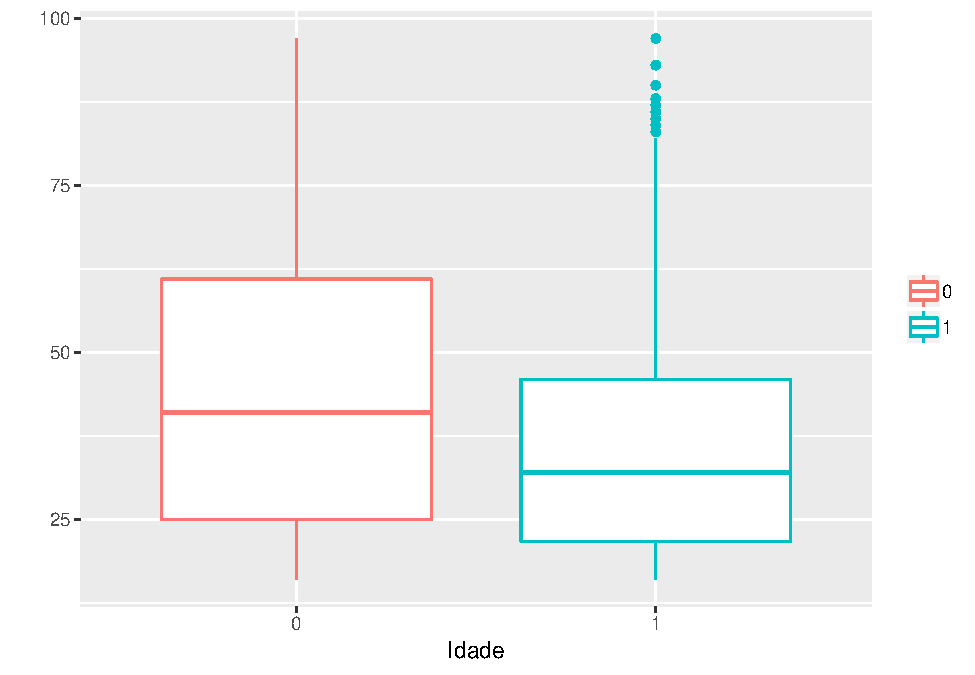
\includegraphics{Binarios_files/figure-latex/unnamed-chunk-7-1.pdf}

\textbf{2.3 Gráficos de frequencia}

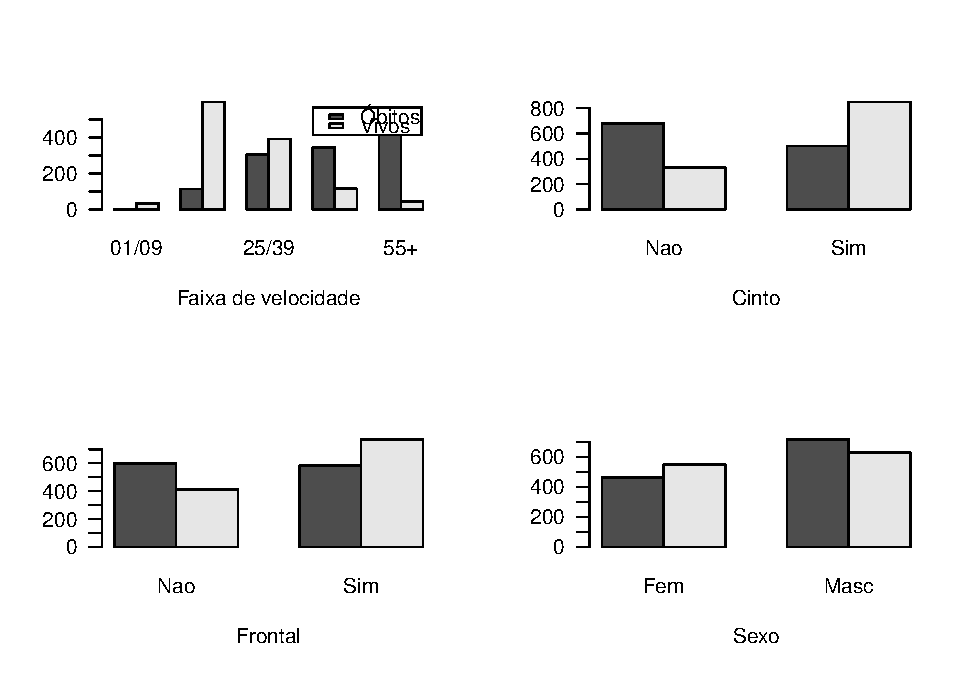
\includegraphics{Binarios_files/figure-latex/unnamed-chunk-8-1.pdf}

\#\#\#Intuitivamente sabemos que para nosso escopo a variável idade não
é significativa para o nosso modelo porém para comprovar adiante faremos
um teste para evidênciar a irrelevancia da variável no modelo.

\hypertarget{ajuste-do-modelo-de-regressao}{%
\section{3. Ajuste do Modelo de
Regressão}\label{ajuste-do-modelo-de-regressao}}

\#\#\textbf{3.1 Ligação Logito}

Vamos ajustar um Modelo Linear Generalizado Binomial com função de
ligação Logito. A expressão do modelo é dada por:

\(ln (\frac{\pi_i}{1-\pi_i}) = \beta_0 + \beta_1 Veloc_i + \beta_2 Sobrev_i + \beta_3 AbFunc_i + \beta_4 Cinto_i + \beta_5 Frontal_i + \beta_6 Sexo_i + \beta_7 Idade_i + \beta_8 Ocupantes_i + \beta_9 Grav_i\)

No R, o modelo é declarado da seguinte forma:

\#\#\textbf{3.2 Ligação Probito}

Vamos ajustar um Modelo Linear Generalizado Binomial com função de
ligação Probito. A expressão do modelo é dada por:

\(\phi^{-1} (\pi_i) = \beta_0 + \beta_1 Veloc_i + \beta_2 Sobrev_i + \beta_3 AbFunc_i + \beta_4 Cinto_i + \beta_5 Frontal_i + \beta_6 Sexo_i + \beta_7 Idade_i + \beta_8 Ocupantes_i + \beta_9 Grav_i\)

No R, o modelo é declarado da seguinte forma:

\begin{Shaded}
\begin{Highlighting}[]
\NormalTok{ajuste2 <-}\StringTok{ }\KeywordTok{glm}\NormalTok{(sobrev }\OperatorTok{~}\StringTok{ }\NormalTok{.,}\DataTypeTok{family=}\KeywordTok{binomial}\NormalTok{(}\DataTypeTok{link =} \StringTok{'probit'}\NormalTok{),}\DataTypeTok{data =}\NormalTok{ dados)}
\end{Highlighting}
\end{Shaded}

\#\#\textbf{3.3 Ligação Complemento log-log}

Vamos ajustar um Modelo Linear Generalizado Binomial com função de
ligação Complemento Log Log. A expressão do modelo é dada por:

\(ln[-ln(1-\pi_i)] = \beta_0 + \beta_1 Veloc_i + \beta_2 Sobrev_i + \beta_3 AbFunc_i + \beta_4 Cinto_i + \beta_5 Frontal_i + \beta_6 Sexo_i + \beta_7 Idade_i + \beta_8 Ocupantes_i + \beta_9 Grav_i\)

No R, o modelo é declarado da seguinte forma:

\begin{Shaded}
\begin{Highlighting}[]
\NormalTok{ajuste3 <-}\StringTok{ }\KeywordTok{glm}\NormalTok{(sobrev }\OperatorTok{~}\StringTok{ }\NormalTok{.,}\DataTypeTok{family=}\KeywordTok{binomial}\NormalTok{(}\DataTypeTok{link=}\StringTok{'cloglog'}\NormalTok{),}\DataTypeTok{data =}\NormalTok{ dados)}
\end{Highlighting}
\end{Shaded}

\#\#\textbf{3.4 Ligação Cauchy}

Vamos ajustar um Modelo Linear Generalizado Binomial com função de
ligação Cauchy. A expressão do modelo é dada por:

\(tan[\pi_i(\mu_i- 0,5)] = \beta_0 + \beta_1 Veloc_i + \beta_2 Sobrev_i + \beta_3 AbFunc_i + \beta_4 Cinto_i + \beta_5 Frontal_i + \beta_6 Sexo_i + \beta_7 Idade_i + \beta_8 Ocupantes_i + \beta_9 Grav_i\)

No R, o modelo é declarado da seguinte forma:

\begin{Shaded}
\begin{Highlighting}[]
\NormalTok{ajuste4 <-}\StringTok{ }\KeywordTok{glm}\NormalTok{(sobrev }\OperatorTok{~}\StringTok{ }\NormalTok{.,}\DataTypeTok{control=}\KeywordTok{glm.control}\NormalTok{(}\DataTypeTok{epsilon =} \FloatTok{1e-8}\NormalTok{, }\DataTypeTok{maxit =} \DecValTok{42}\NormalTok{, }
                                           \DataTypeTok{trace =} \OtherTok{FALSE}\NormalTok{), }\DataTypeTok{family=}\KeywordTok{binomial}\NormalTok{(}\DataTypeTok{link=}\StringTok{'cauchit'}\NormalTok{),}\DataTypeTok{data =}\NormalTok{ dados)}
\end{Highlighting}
\end{Shaded}

\hypertarget{escolha-do-modelo}{%
\section{4. Escolha do Modelo}\label{escolha-do-modelo}}

O critério de informação AIC pode também ser utilizado, porém o AIC
penaliza o número de parâmetros do modelo. Como os modelos tem o mesmo
número de parâmetros, o critério aponta para a mesma direção da
verossimilhança pois todos são penalizados da mesma forma.

O modelo que apresentou menor AIC e maior verossimilhança foi o modelo
Binomial com função de ligação Cauchy.

\hypertarget{analise-do-modelo-ajustado-selecionado}{%
\section{5. Análise do Modelo Ajustado
Selecionado}\label{analise-do-modelo-ajustado-selecionado}}

\#\#\textbf{5.1 Resumo do Modelo}

LIneu O resumo do modelo ajustado indica que as variáveis adesão
marginal, nucléolos nus, cromatina branda, nucléolo normal e espessura
do aglomerado estão associadas a uma maior probabilidade de tumor
maligno, enquanto as demais variáveis não apresentam relação com a
resposta.

\#\#\textbf{5.2 Reajuste do Modelo}

Lineu Como as covariáveis são altamente correlacionadas, é válido
inserir as covariáveis uma a uma no modelo para verificar sua
significância na presença das outras, tal como o realizado pelo
algoritmo stepwise.

Sendo assim, o novo modelo fica da seguinte forma:

\begin{Shaded}
\begin{Highlighting}[]
\NormalTok{ajuste4}\FloatTok{.1}\NormalTok{ <-}\StringTok{ }\KeywordTok{step}\NormalTok{(ajuste4, }\DataTypeTok{direction =} \StringTok{"both"}\NormalTok{)}
\end{Highlighting}
\end{Shaded}

O resumo do novo modelo ajustado:

\begin{Shaded}
\begin{Highlighting}[]
\KeywordTok{anova}\NormalTok{(ajuste4, ajuste4}\FloatTok{.1}\NormalTok{, }\DataTypeTok{test =} \StringTok{'Chisq'}\NormalTok{)}
\end{Highlighting}
\end{Shaded}

\begin{verbatim}
## Analysis of Deviance Table
## 
## Model 1: sobrev ~ veloc + cinto + frontal + sexo + idade + ocupantes + 
##     abfunc
## Model 2: sobrev ~ veloc + cinto + frontal + sexo + idade + ocupantes
##   Resid. Df Resid. Dev Df Deviance Pr(>Chi)
## 1      2349     2018.1                     
## 2      2350     2019.4 -1  -1.2619   0.2613
\end{verbatim}

\#\#\textbf{5.3 Análise de Resíduos}

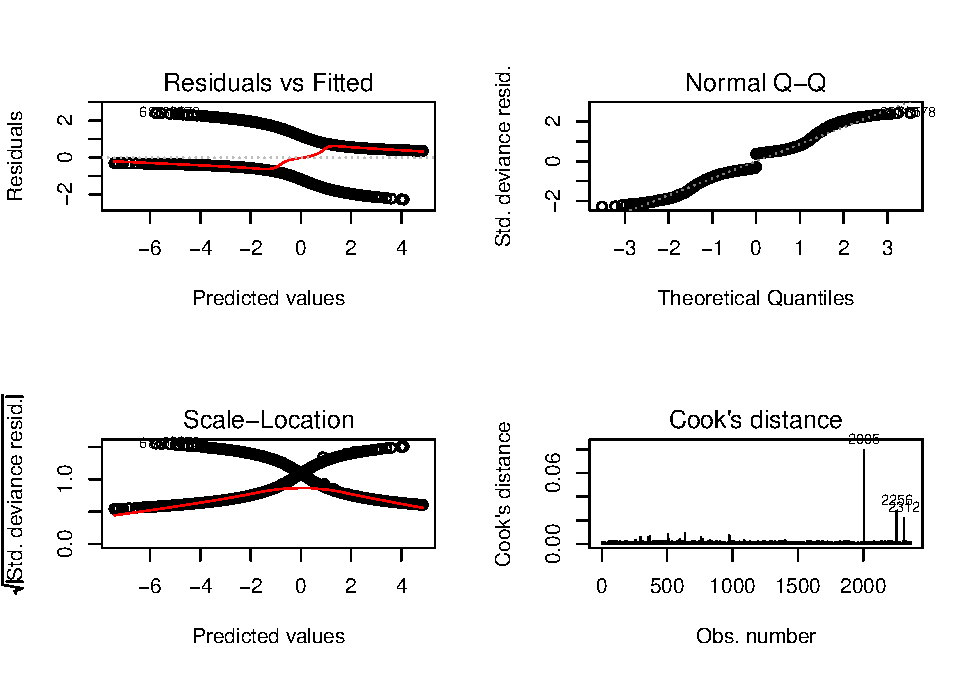
\includegraphics{Binarios_files/figure-latex/unnamed-chunk-18-1.pdf}
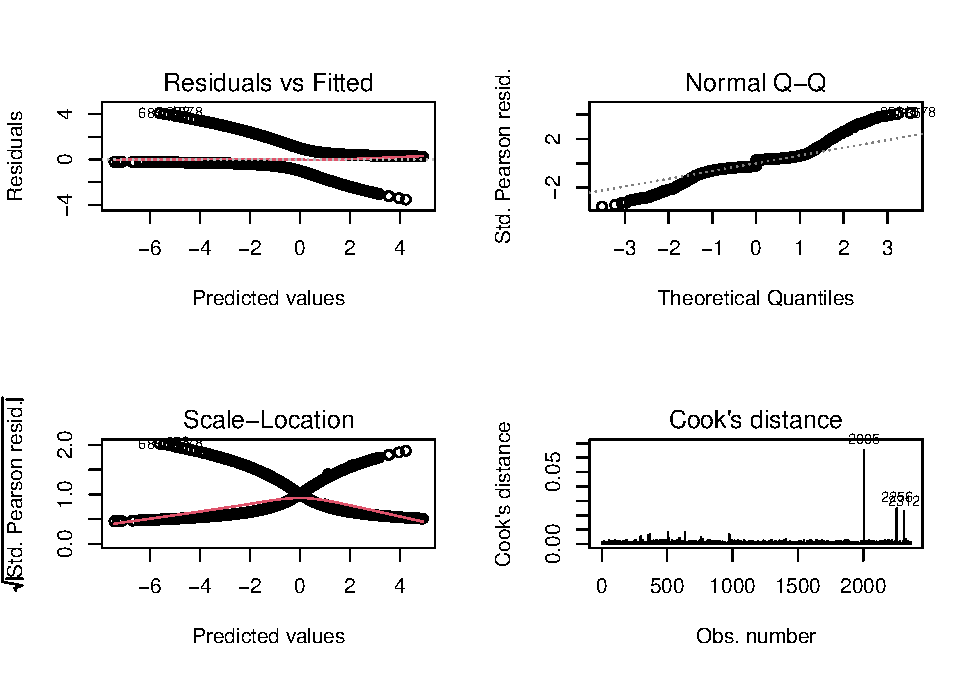
\includegraphics{Binarios_files/figure-latex/unnamed-chunk-18-2.pdf}

\textbf{5.4 Medidas de Influencia}

\begin{Shaded}
\begin{Highlighting}[]
\KeywordTok{influenceIndexPlot}\NormalTok{(ajuste4}\FloatTok{.1}\NormalTok{, }\DataTypeTok{vars=}\KeywordTok{c}\NormalTok{(}\StringTok{"Cook"}\NormalTok{), }\DataTypeTok{main=}\StringTok{"Distância de Cook"}\NormalTok{)}
\end{Highlighting}
\end{Shaded}

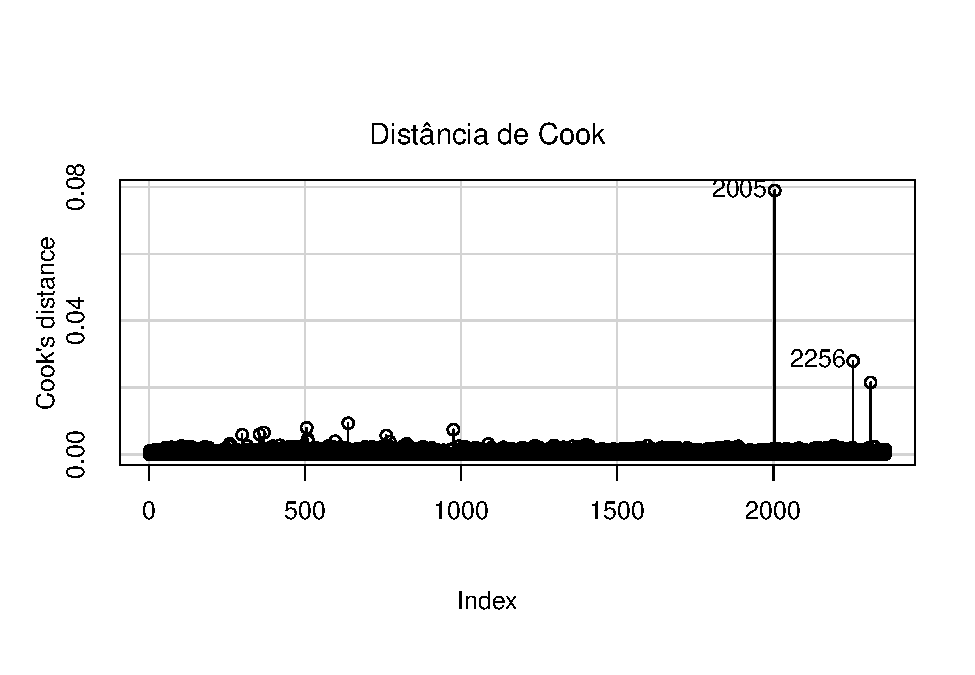
\includegraphics{Binarios_files/figure-latex/unnamed-chunk-19-1.pdf}

\begin{Shaded}
\begin{Highlighting}[]
\KeywordTok{influenceIndexPlot}\NormalTok{(ajuste4}\FloatTok{.1}\NormalTok{, }\DataTypeTok{vars=}\KeywordTok{c}\NormalTok{(}\StringTok{"Studentized"}\NormalTok{), }\DataTypeTok{main=}\StringTok{"Resíduos Padronizados"}\NormalTok{)}
\end{Highlighting}
\end{Shaded}

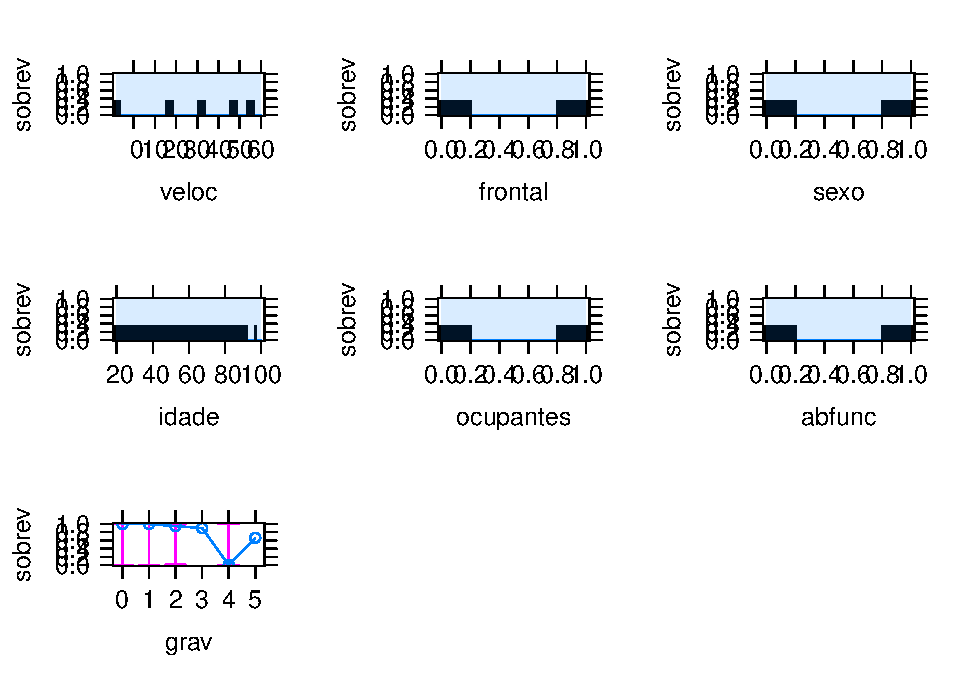
\includegraphics{Binarios_files/figure-latex/unnamed-chunk-20-1.pdf}

\textbf{5.5 Resíduos Quantílicos Aleatoriazados}

\#\#\textbf{5.6 Gráfico Normal de Probabilidades com Envelope Simulado}

Lineu O gráfico de resíduos simulados permite verificar a adequação do
modelo ajustado mesmo que os resíduos não tenham uma aproximação
adequada com a distribuição Normal. Neste tipo de gráfico espera-se,
para um modelo bem ajustado, os pontos (resíduos) dispersos
aleatoriamente entre os limites do envelope.

Deve-se ficar atento à presença de pontos fora dos limites do envelope
ou ainda a pontos dentro dos limites porém apresentando padrões
sistemáticos.

Vamos utilizar a função envelope implementada pelo professor Cesar
Augusto Taconeli :

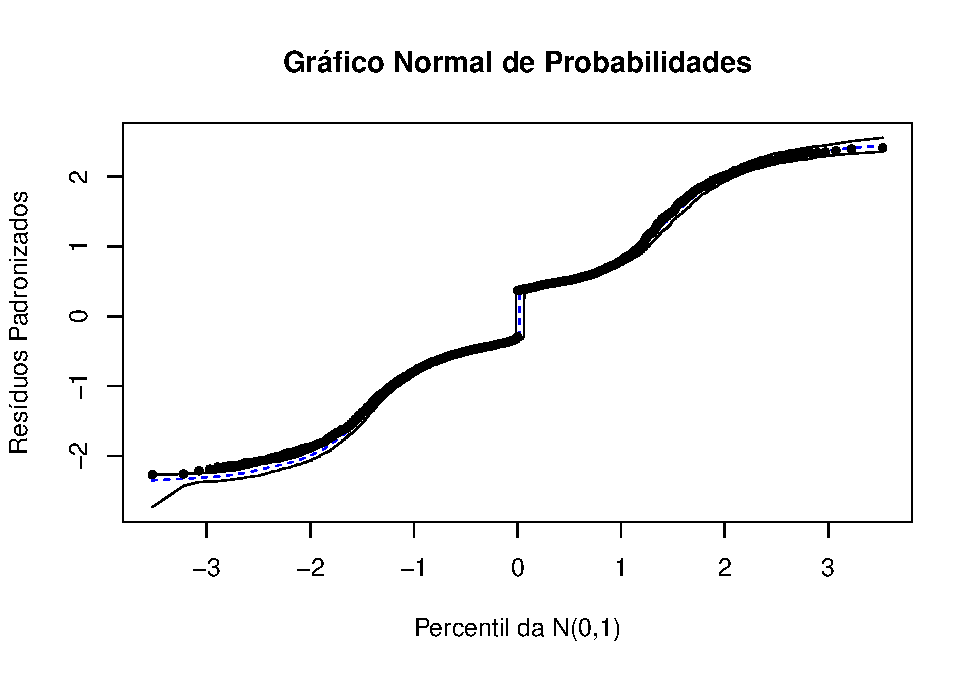
\includegraphics{Binarios_files/figure-latex/unnamed-chunk-21-1.pdf}

\textbf{5.7 Gráficos de Efeitos}

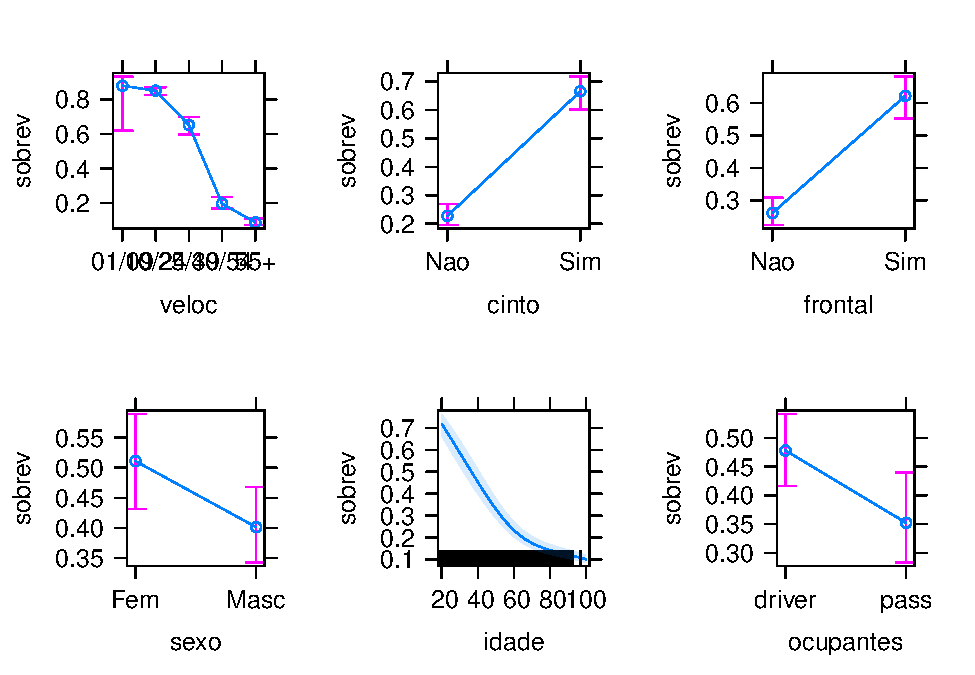
\includegraphics{Binarios_files/figure-latex/unnamed-chunk-22-1.pdf}

\hypertarget{predicao}{%
\section{6. PREDIÇÃO}\label{predicao}}

\hypertarget{avaliacao-do-poder-preditivo-do-modelo}{%
\section{7. AVALIAÇÃO DO PODER PREDITIVO DO
MODELO}\label{avaliacao-do-poder-preditivo-do-modelo}}

Como temos uma base de tamanho razoável para fins preditivos, uma
alternativa é separar a base em duas: uma para o ajuste do modelo, com
70\% dos dados (com 477 observações) e outra para validação, com 30\%
(com 203 observações).

\hypertarget{divisao-da-base-de-dados}{%
\subsection{\texorpdfstring{\textbf{7.1 Divisão da Base de
dados}}{7.1 Divisão da Base de dados}}\label{divisao-da-base-de-dados}}

\begin{Shaded}
\begin{Highlighting}[]
\KeywordTok{set.seed}\NormalTok{(}\DecValTok{1909}\NormalTok{)}
\NormalTok{indices <-}\StringTok{ }\KeywordTok{sample}\NormalTok{(}\DecValTok{1}\OperatorTok{:}\DecValTok{680}\NormalTok{, }\DataTypeTok{size =} \DecValTok{477}\NormalTok{) }
\NormalTok{dadosajuste <-}\StringTok{ }\NormalTok{dados[indices,]}
\NormalTok{dadosvalid <-}\StringTok{ }\NormalTok{dados[}\OperatorTok{-}\NormalTok{indices,]}
\end{Highlighting}
\end{Shaded}

\hypertarget{ponto-de-corte}{%
\subsection{\texorpdfstring{\textbf{7.2 Ponto de
Corte}}{7.2 Ponto de Corte}}\label{ponto-de-corte}}

Como estamos modelando a probabilidade de tumor maligno, vamos
estabelecer o ponto de corte 0.5, isso é, se a probabilidade estimada
for maior que este valor o tumor será classificado como maligno. Vamos
armazenar os valores preditos do modelo para os dados de validação:

\begin{Shaded}
\begin{Highlighting}[]
\NormalTok{pred <-}\StringTok{ }\KeywordTok{predict}\NormalTok{(ajuste4}\FloatTok{.1}\NormalTok{, }\DataTypeTok{newdata =}\NormalTok{ dadosvalid, }\DataTypeTok{type =} \StringTok{'response'}\NormalTok{)}
\NormalTok{corte <-}\StringTok{ }\KeywordTok{ifelse}\NormalTok{(pred }\OperatorTok{>}\StringTok{ }\FloatTok{0.5}\NormalTok{, }\StringTok{'maligno'}\NormalTok{, }\StringTok{'benigno'}\NormalTok{)}
\end{Highlighting}
\end{Shaded}

\textbf{7.3 Sensibilidade e Especificidade}

Para fazer uso dos dados de validação, dois conceitos são necessários:
sensibilidade e especificidade.

Define-se por sensibilidade a capacidade do modelo de detectar tumores
malignos, ou seja, de classificar como malignos os tumores que de fato o
são .

Já a especificidade é a capacidade do modelo de detectar classificar
como benignos tumores verdadeiramente benignos.

A sensibilidade é dada por

\begin{Shaded}
\begin{Highlighting}[]
\CommentTok{#sens <- dados[2,2]/sum(dados[,2])}
\CommentTok{#sens }
\end{Highlighting}
\end{Shaded}

\textbf{7.4 Curva ROC}

\textbf{7.5 Outra Alternativa de validação}

\hypertarget{referencias}{%
\section{8. REFERÊNCIAS}\label{referencias}}


\end{document}
